\documentclass[xetex]{scrartcl}

% packages
\usepackage{xltxtra}
\usepackage{polyglossia}
\usepackage{lsalike}
\usepackage{hyperref}
\usepackage{fontspec}
\usepackage{covington}
\usepackage{scrpage2}
\usepackage{qtree}
\usepackage[left=2.5cm,right=2.5cm,top=3.5cm,bottom=3.5cm]{geometry}
\usepackage{hieroglf}
\usepackage[weather,misc,alpine]{ifsym}
\usepackage{pst-node}
\usepackage{colortbl}
\usepackage{alltt}
\usepackage{listings}
\usepackage{multirow}

% fonts general
\setmainfont[Mapping=tex-text,Scale=1.0]{FreeSans}
\setsansfont[Mapping=tex-text,Scale=1.0]{FreeSans}
\setmonofont{FreeMono}

% special fonts
\newfontfamily\hana{HAN NOM A}
\newfontfamily\hanb{HAN NOM B}
\newfontfamily\sil{Charis SIL}
\newfontfamily\grk{Aristarcoj}
\newfontfamily\calligraphy{Chinese Calligraphy}
\newfontfamily\pur{Purisa}


\newcommand{\White}[1]{\cellcolor{white} \textcolor{black}{ #1}}

% language settings
\setmainlanguage[spelling=new]{german}
\setotherlanguage{english}

% pagestyle settings
\pagestyle{scrheadings}
\ihead{Johann-Mattis List}
\chead{CALC Seminar}
\ohead{2018-04-10}
\ifoot{}
\cfoot{\pagemark}
\ofoot{}



\begin{document}
%\maketitle

\begin{center}
    {\bf \huge  Introduction to Computer-Assisted Language Comparison}
\end{center}

\section{Introduction}\label{introduction}

By comparing the languages of the world, we gain invaluable insights
into human prehistory and cognition. The traditional methods for
language comparison are based on manual data inspection. With more and
more data available, they reach their practical limits. Computer
applications, however, are not capable of replacing experts' experience
and intuition. In a situation where computers cannot replace experts and
experts do not have enough time to analyse the massive amounts of data,
a new framework, neither completely computer-driven, nor ignorant of the
help computers provide, becomes urgent. Such frameworks are
well-established in biology and translation, where computational tools
cannot provide the accuracy needed to arrive at convincing results, but
do assist humans to digest large data sets.

The seminar will provide a basic introduction into the major ideas
behind the framework of Computer-Assisted Language Comparison (CALC)
which is currently actively being developed. This framework pursues an
interdisciplinary approach that adapts methods from computer science and
bioinformatics for the use in historical linguistics. While purely
computational approaches are common today, we focus on the communication
between classical and computational linguists, developing interfaces
that allow linguists to produce their data in machine readable formats
while at the same time presenting the results of computational analyses
in a transparent and human-readable way.

While our seminar does not require initial knowledge in programming, we
assume that our participants have basic knowledge of topics in
historical linguistics. It is clear that we cannot offer a full-fledged
tutorial in programming. So we rely on the readiness of our participants
to catch up with certain problems by searching the web. Regarding
specific topics in historical linguistics, we plan to give concise
theoretical introductions, to make sure all participants are on the same
page. But here as well, we hope that participants are ready to read some
of the literature we reference in order to catch up in those cases
exceeding their expertise.

\section{Seminar Website and GitHub
Account}\label{seminar-website-and-github-account}

Our seminar is accompanied by a seminar website where you find links to
all handouts for each session. The website is availabe at
\url{http://calc.digling.org/seminar/}. We also use a GitHub repository
to collect questions of seminar participants and to share the data and
additional information accompanying the seminar. The GitHub repository
can be found at \url{https://github.com/digling/calc-seminar/}. We ask
all participants to acquaintain themselves with the concept of
\href{https://github.com/digling/calc-seminar/issues}{issues} on GitHub,
as this is the preferred format we want to use for communication if
participants have additional questions (emails can still be written to
us, but we prefer open questions of which it is useful for all
participants to have an answer to be posted in form of issues on
GitHub).

\section{Schedule for the Seminar}\label{schedule-for-the-seminar}
\begin{center}
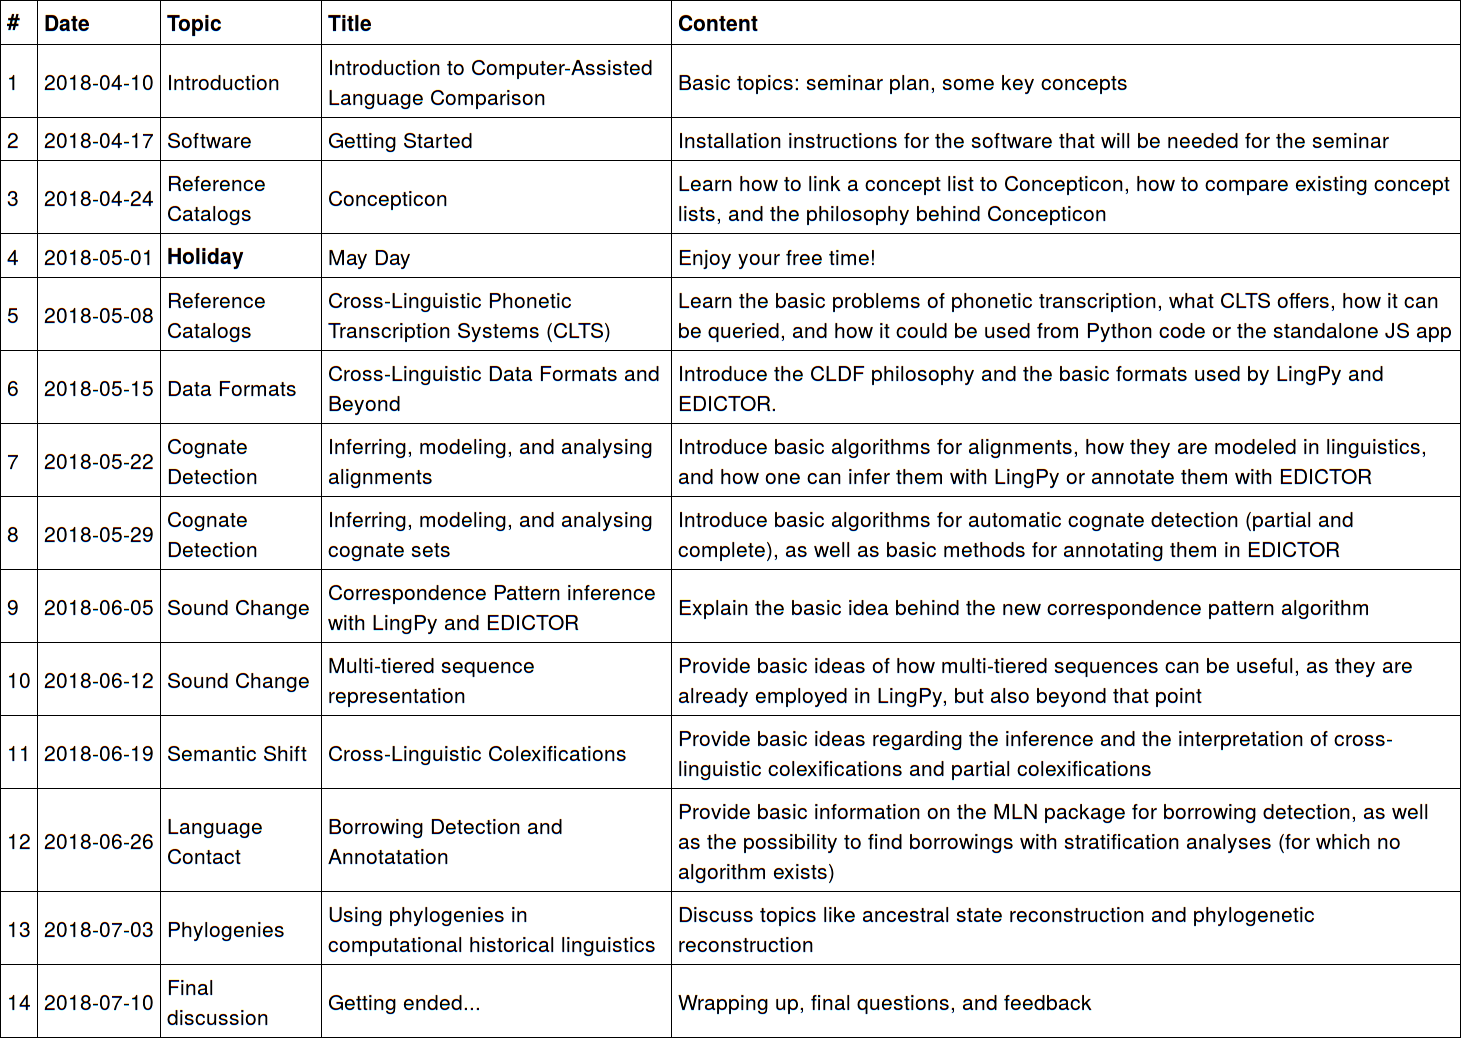
\includegraphics[width=\textwidth]{img/s1-table.png}
\end{center}

\section{Structure of the Sessions}\label{structure-of-the-sessions}

The sessions will be structured in a rather free form. Each session is
accompanied by a so-called \href{http://jupyter.org/}{Jupyter Notebook}.
These allow to follow tutorials both by inspecting the static code, but
also interactively, provided one has installed the notebook software
available from the Jupyter project. Each ``handout'' we provide is in
fact a notebook, and it can both be read in form of printed paper or an
electronic version of it, or studied interactively. Information on how
to install Jupyter notebooks will be provided during the second session
of the seminar.

We may occasionally, but not necessarily always, start with a
theoretical background before looking at the coding examples. Having
grasped the tasks at hand theoretically may be quite important. Since we
do not yet know to which degree our course members are proficient in the
basic topics of historical linguistics, we encourage all members of the
seminar to raise questions in case some terminology we use is opaque or
unknown to them.

We do not give any homework, nor do we plan on providiging too many
tasks during the seminar. Instead we encourage all participants to
either follow the notebooks directly during the sessions when we
introduce them, or to test them at home. We may occasionally ask
participants to solve some exercises, but we do not necessarily prepare
exercises for all sessions. We encourage all participants to contact us
inbetween the different sessions with their individual questions they
may have.

We offer, in addition, that participants present data-driven projects
they are working on during our seminar, where they describe the problems
they have to solve, and all participants as well as the seminar leaders
try to discuss whether simple solutions can be found with the tools
available for us.

\section{Computer-Assisted Language Comparison in a
Nutshell}\label{computer-assisted-language-comparison-in-a-nutshell}

As mentioned above, both pure classical approaches and pure
computational approaches in historical linguistics have their specific
shortcomings. The former lack efficiency, since they are are carried out
manually, which makes their application time-consuming and tedious, but
they also lack consistency, since they are not based on formal
guidelines. The latter lack flexibility (being only applicable to
certain datasets and questions) and accuracy (compared to manual
analyses). In addition, they often still rely on manually annotated
data, and they produce results in a black-box fashion, making it
difficult for scholars to inspect them.

If we combine classical with computational approaches, however, we can
single out their advantages and disadvantages. Computattional approaches
offer consistency and efficiency, while classical approaches can add
accuracy and flexibility. Combining both approaches within a
computer-assisted as opposed to a computer-based or a computer-less
framework will therefore greatly benefit the research in the field of
historical language comparison.

This is the basic idea behind the CALC approach. But to implement this
idea, one needs to find good ways to allow humans to communicate with
machines and \emph{vice versa}. The approach we follow in CALC is to
base the analysis on three different building blocks, namely the
\emph{data}, which should be available in human- and machine-readable
form, the \emph{software} which analyses the data, and the
\emph{interfaces} which allow scholars to inspect the results produced
by the software and to produce and modify the data. This is represented
in the following illustration.

\begin{figure}[htbp]
\centering
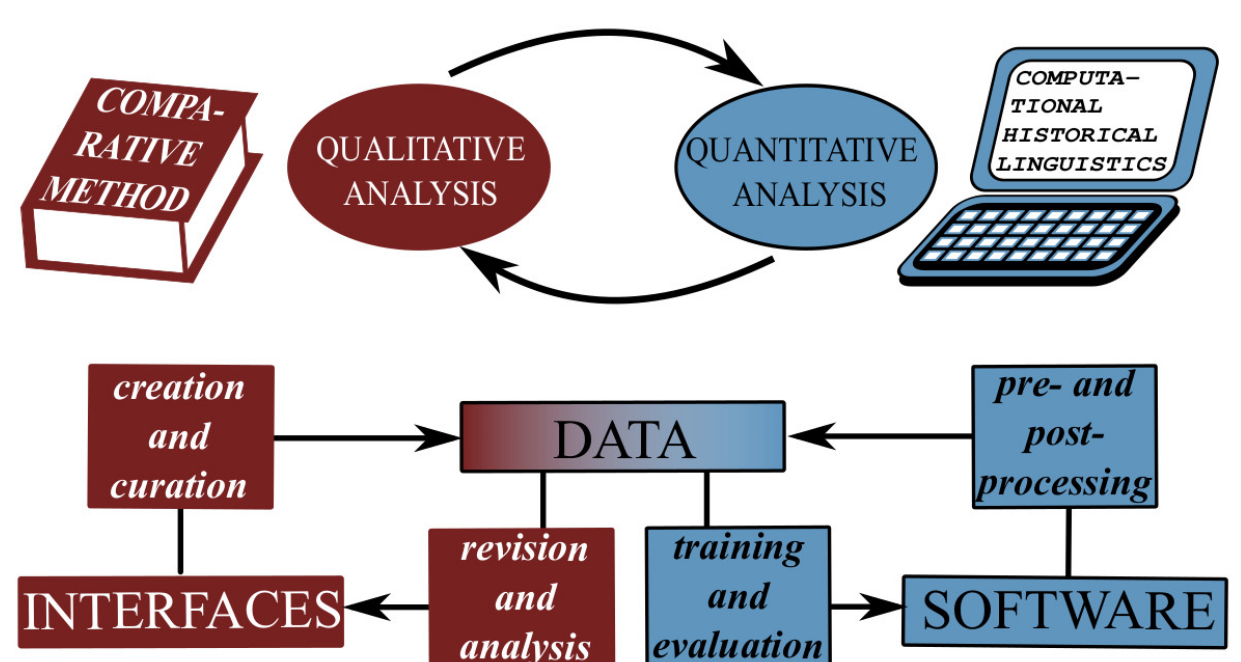
\includegraphics[width=\textwidth]{img/s1-calc.png}
\caption{image}
\end{figure}

During the seminar, we will introduce these different aspects in more
detail. Having installed the software (Session 2), we will first turn to
the data by introducing the concept of \emph{reference catalogs}
(Sessions 3 and 4), and the major idea behind the \emph{cross-linguistic
data formats} initiative (Session 5, \url{http://cldf.clld.org}). We
will then turn to software and interfaces that help us to search for
cognates across multilingual datasets (Sessions 6 and 7). Cognates are
words that share a common history, and we will show how one can identify
them both manually and automatically. The basis for cognate detection is
the fact that \emph{sound change} proceeds in some seemingly regular
fashion. We will try to explore this further by introducing a method for
the identification of \emph{sound correspondence patterns} in
multilingual datasets (Session 9), and by introducing the idea of
\emph{multi-tiered sequence representation}, a specific way of
annotating data which helps us to model how sounds change from an
ancestral to its descendant languages (Session 10). \emph{Semantic
shift} is another important topic in historical linguistics, and we
cover it by discussing the idea of \emph{cross-linguistic
colexifications} which can give us initial hints on general patterns of
recurring polysemies across the languages of the world (Session 11). The
detection of \emph{borrowings} in linguistic datasets is notoriously
difficult. We will nevertheless try to introduce at least one simple
approach and the (so far not implemented) method that linguists use in
order to infer borrowings manually (Session 12). In the last thematic
session, we will briefly discuss different methods related to
phylogenies (family trees) of languages (Session 13). The seminar will
then be completed by a final discussion session where we ask the
participants for their feedback and experience (Session 14).


%\section*{Literatur}
%\bibliographystyle{lsalike}
%\renewcommand\refname{Literatur}
\renewcommand{\section}[2]{}
%\bibliography{/home/mattis/Dropbox/EvoClass/bibliography/evoclass}
\end{document}

